\section{Variational Approach for Determination of the Eigenvalues of \eqref{eq:SI-WaveEqn}} \label{sec:SI-VarProbMethod}
As mentioned in section \ref{sec:SI-ProblemFormulation}, the fact that $-\laplacian_{\ccompMes}^\qm$ is self-adjoint for each $\qm$, combined with use of the min-max principle, implies that the eigenvalues $\omega_{n}^2$ (and eigenfunctions $u_n$) of $-\laplacian_{\ccompMes}^\qm$ are the minimum values (respectively minimisers) of the following variational problem:
\begin{align} \label{eq:SI-VarProb}
	\omega_n^2 &:= \min_{u}\clbracs{ \integral{\ddom}{ \abs{\tgrad_{\ccompMes}u}^2 }{\ccompMes} \setVert \norm{u}_{\ltwo{\ddom}{\ccompMes}}=1, \ \ip{u}{u^{(l)}}_{\ltwo{\ddom}{\dddmes}}=0 \ \forall 1\leq l\leq n-1 },
\end{align} 
where the eigenvalues (and their corresponding eigenfunctions) are numbered in ascending order.
Our interest is in determining the eigenvalues $\omega_n^2$, however we also need to determine the eigenfunctions $u_n$ since $u_{n-1}$ through $u_1$ are required for computation of $u_{n}$.
Since we can obtain the eigenvalue $\omega_n^2$ from the eigenfunction $u_n$, by evaluating the integral in \eqref{eq:SI-VarProb}, we will focus our discussion on the approximation (and computation) of the eigenfunctions.
We also drop the explicit subscript $n$, and just consider the problem of determining the function $u\in\tgradSob{\ddom}{\ccompMes}$ which solves the optimisation problem;
\begin{subequations} \label{eq:SI-MinProblem}
	\begin{align}
		\text{Minimise} \quad & \quad \integral{\ddom}{ \abs{\tgrad_{\ccompMes}u}^2 }{\ccompMes} \\
		\text{Subject to} \quad & \quad \integral{\ddom}{ \abs{u}^2 }{\ccompMes} = 1, \\
		& \quad \integral{\ddom}{ u\cdot\overline{u}^{(l)} }{\ccompMes} = 0, \ 1\leq l\leq n-1,
	\end{align}
\end{subequations}
where $n\in\naturals$, $u^{(l)}, 1\leq l\leq n-1$ are a finite list of (given) orthonormal functions.

The traditional idea when attempting to approximate a minimising function is to select a finite-dimensional subspace of the solution space ($\tgradSob{\ddom}{\ccompMes}$ in this case), and then find the best approximation to the minimising function $u$ in this space.
For example, we could elect to represent the minimising function $u$ in terms of a basis $\clbracs{\varphi_m}_{m\in\naturals_0}$ for $\tgradSob{\ddom}{\ccompMes}$, truncate the basis expansion at some index $M$,
\begin{align} \label{eq:SI-VPTruncatedBasis}
	u &\approx \sum_{m=0}^M u_m \varphi_m,
\end{align}
and solve the minimisation problem (that arises from substituting \eqref{eq:SI-VPTruncatedBasis} into \eqref{eq:SI-MinProblem}) in the coefficients of the basis expansion $\clbracs{u_m}_{1\leq m\leq M}$.
This minimisation problem will be discrete (solving for the $M+1$ independent variables $u_m$) and can be handled using optimisation methods, with the choice of $\varphi_m$ and $M$ affecting the accuracy of the approximate eigenfunction (and eigenvalue).
We can look to apply these ideas to the problem \eqref{eq:SI-MinProblem}.

Our first task is to decide on the finite-dimensional subspace and/or the basis functions $\varphi_m$ that we want to use to approximate $u$.
From the standpoint of accuracy (and typically speed of computation) of the numerical solution there are a number of properties that it is desirable for this basis to have; orthonormality between the $\varphi_m$, similar shape to that expected of $u$, and a quantifiable rate of decay of the coefficients $u_m$.
This is where the unfamiliar nature of our space $\tgradSob{\ddom}{\ccompMes}$ begins to cause problems as the choices we have for such bases are considerably more complex --- choosing the behaviour of $\varphi_m$ in the bulk regions then restricts what $\varphi_m$ can do on the skeleton, and vice-versa. 
The geometry of the skeleton can also compound this issue, particularly if there are a large number of bulk regions $\ddom_i$, if their shapes are significantly different (in terms of size or layout) from each other, or there are a small number of irregularly shaped bulk regions.
In such settings one could consider choosing ``local" basis functions in similar fashion to finite element schemes; mesh the domain $\ddom$ into a union of simplexes (usually triangles) by placing nodes $\tau_i\in\ddom$, and use ``tent" (or ``hat") functions\footnote{These are functions that are equal to unity at a given node $\tau_i$, decay to zero on the simplexes that have $\tau_i$ as a node, and are zero on the rest of $\ddom$.} centred on each node $\tau_i$ for the truncated basis functions $\varphi_m$.
This allows sufficient flexibility in the behaviour of $u$ on the edges and in the bulk regions, at the expense of requiring a new mesh for every new graph geometry.
We will continue this train of thought in our discussion in section \ref{sec:SI-Conc}.

Fortunately, the geometry of our cross-in-the-plane example is rather simple, since the two edges $I_h, I_v$ are aligned with the coordinate axes.
This makes computing integrals on the skeleton and traces from the bulk region relatively simple (compared to more general geometries), so we can avoid taking the approach of meshing $\ddom$ as described above.
Instead we can opt to choose a basis in a way more akin to spectral methods --- by choosing ``global" basis functions rather than the ``local" basis functions described above.
Combined with the fact that we only have one bulk region that spans the entire period cell, the natural candidate for our basis functions would be the 2D Fourier basis $\e^{2\pi\rmi(\alpha x + \beta y)}$.
These functions are orthogonal in $\ltwo{\ddom}{\compMes}$, however are not orthogonal in $\ltwo{\ddom}{\ccompMes}$ --- the inner product of two distinct functions is exactly $\alpha_0$.
This on its own does not prevent us from utilising these functions as a basis; however they also possess a continuous (in the sense of matching traces) normal derivative across the skeleton, which functions in $\tgradSob{\ddom}{\ccompMes}$ are not required to have\footnote{We will later see in section \ref{sec:SI-StrongDerivation} exactly how this potential mismatch in the traces of the normal derivative affects the eigenfunctions.}.
Instead we use periodic, two-dimensional polynomials to approximate our function $u$, by taking an order $M\in\naturals$ and setting
\begin{align} \label{eq:2DPolyBasisDef}
	\varphi_m(x,y) &= x^{i_m} y^{j_m}, \quad m = j_m + Mi_m, \ i,j\in\clbracs{0,...,M-1},
\end{align}
and imposing the periodicity constraint that
\begin{align*}
	u\bracs{0,y} = u\bracs{1,y}, \ \forall y\in\sqbracs{0,1}, 
	\qquad 
	u\bracs{x,0} = u\bracs{x,1}, \ \forall x\in\sqbracs{0,1}.
\end{align*}
This is a suitable finite-dimensional subspace for $\tgradSob{\ddom}{\ccompMes}$ in which to approximate $u$; two dimensional (periodic) polynomials are dense in $\tgradSob{\ddom}{\lambda_2}$, and since we have that functions $u\in\tgradSob{\ddom}{\ccompMes}$ are continuous across the skeleton, the trace of such polynomials also approximates $u$ on the skeleton.
We also know that $u$ is continuous at the vertices, which such polynomial approximations provide, but they also do not enforce matching normal derivative traces across the skeleton.
In the case where one has multiple bulk regions, one can build on this idea by approximating with ``piecewise polynomials" --- approximate via a polynomial basis on each bulk region $\ddom_i$, then impose that the approximations must coincide on any part of the skeleton common to the boundary of two bulk regions.

With our choice of polynomial basis, and writing $U = \bracs{u_0,...,u_{M^2-1}}^\top$, we are tasked with solving the following problem for our cross in the plane geometry.
\begin{problem}[Discrete Variational Problem] \label{prob:DiscVarProb}
	Let $M,N\in\naturals$ and $\varphi_m$ be as in \eqref{eq:2DPolyBasisDef}.
	Given coefficients $U_l=\bracs{u^l_0,...,u^l_{M^2-1}}^\top$ for $1\leq l\neq N-1$, find values $U=\bracs{u_0,...,u_{M^2-1}}^\top$ that:
	\begin{subequations} \label{eq:SI-ExampleMinProb}
		\begin{align}
			\text{Minimise} \quad & \quad J\sqbracs{U} := \sum_{m=0}^{M^2-1}\sum_{n=0}^{M^2-1}u_m\overline{u}_n\ip{\tgrad_{\ccompMes}\varphi_m}{\tgrad_{\ccompMes}\varphi_n}_{\ltwo{\ddom}{\ccompMes}^2} 
			\label{eq:SI-EMPObjectiveFn} \\
			\text{Subject to} \quad & \quad \sum_{m=0}^{M^2-1}\sum_{n=0}^{M^2-1}u_m\overline{u}_n\ip{\varphi_m}{\varphi_n}_{\ltwo{\ddom}{\compMes}} = 1, 
			\label{eq:SI-EMPNormConstraint} \\
			& \quad \sum_{i_m=1}^{M-1}u_{j_m+Mi_m} = 0, \ \forall j_m\in\clbracs{0,...,M-1}, 
			\label{eq:SI-EMPxPeriodicity} \\
			& \quad \sum_{j_m=1}^{M-1}u_{j_m+Mi_m} = 0, \ \forall i_m\in\clbracs{0,...,M-1},
			\label{eq:SI-EMPyPeriodicity} \\
			& \quad \sum_{m=0}^{M^2-1}\sum_{n=0}^{M^2-1}u_m\overline{u}^l_n\ip{\varphi_m}{\varphi_n}_{\ltwo{\ddom}{\ccompMes}} = 0, \ \forall 1\leq l\leq N-1.
			\label{eq:SI-EMPOrthogonality}
		\end{align}
	\end{subequations}
\end{problem}
The minimiser $U$ of problem \ref{prob:DiscVarProb} then provides our approximation of $u$, and we have that $\omega^2 \approx J[U]$.
Equation \eqref{eq:SI-EMPNormConstraint} is the norm constraint on the eigenfunction $u$, \eqref{eq:SI-EMPxPeriodicity} (respectively \eqref{eq:SI-EMPyPeriodicity}) are the constraints that ensure periodicity of the eigenfunction in the $\widehat{x}_1$ (respectively $\widehat{x}_2$) directions, and \eqref{eq:SI-EMPOrthogonality} forces $u$ to be orthogonal to the previously computed eigenfunctions $u^l$.

A glaring drawback to this method is its sequential nature --- if we want to compute the $n^{\text{th}}$ eigenvalue, then we need to compute each of $u_1,...,u_{n-1}$ too.
Compounding this is that the finite dimension of our problem (through the truncation at order $M$) means that we are only ever able to compute approximations to the lowest $M^2 - \bracs{2M + 1} + 1$ eigenvalues, due to the number of constraints in the problem \ref{prob:DiscVarProb}.
This in particular makes it difficult to examine any part of the spectrum that is far away from zero --- if one does not know \emph{a priori} how the eigenvalues $\omega_n$ scale with $n$, one simply has to continue computing successive eigenvalues until they reach the region of the spectrum they want to explore.
In doing so, one might find that the approximating subspace is of too small a dimension, or might grossly overestimate how large the dimension should be and waste computation time.
This being said, we are able to recover each of the spectral bands (and dispersion relations) in succession, provided we are willing to put in the required computation time and power.
The approximate spectral bands as computed from the problem \ref{prob:DiscVarProb} with $M=12$ and $\alpha=0$ can be viewed in figure \ref{fig:CompositeCross-VP-SpectralBands}.
\begin{figure}[t!]
	\centering
	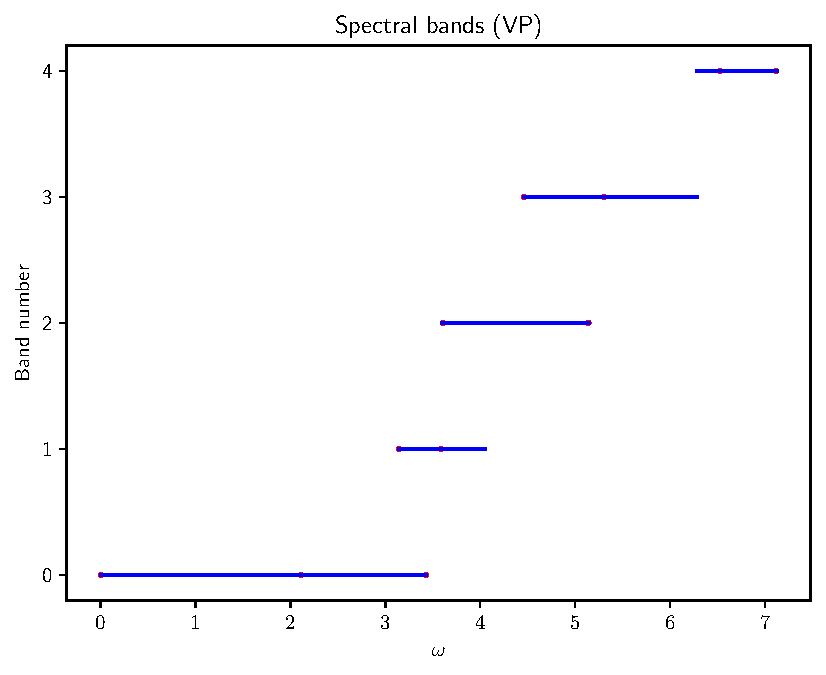
\includegraphics[scale=0.5]{CompositeCross-VP-SpectralBands.pdf}
	\caption[Eigenvalues of \eqref{eq:SI-WaveEqn}, computed via solution of problem \ref{prob:DiscVarProb}.]{\label{fig:CompositeCross-VP-SpectralBands} The eigenvalues belonging to the first 5 bands, approximated via the problem \ref{prob:DiscVarProb}.}
\end{figure}
We remark that there are no gaps between the spectral bands in this case, although gaps do open when $\alpha>0$ --- this will be demonstrated in section \ref{sec:SI-StrongDerivation}.
We can also notice that the eigenvalues within each band obey the symmetries in $\qm$ as expected from proposition \ref{prop:CrossInPlaneSymmetries}, by examining the dispersion relations in figure \ref{fig:VP_AllBands}.
\begin{figure}[t!]
	\centering
	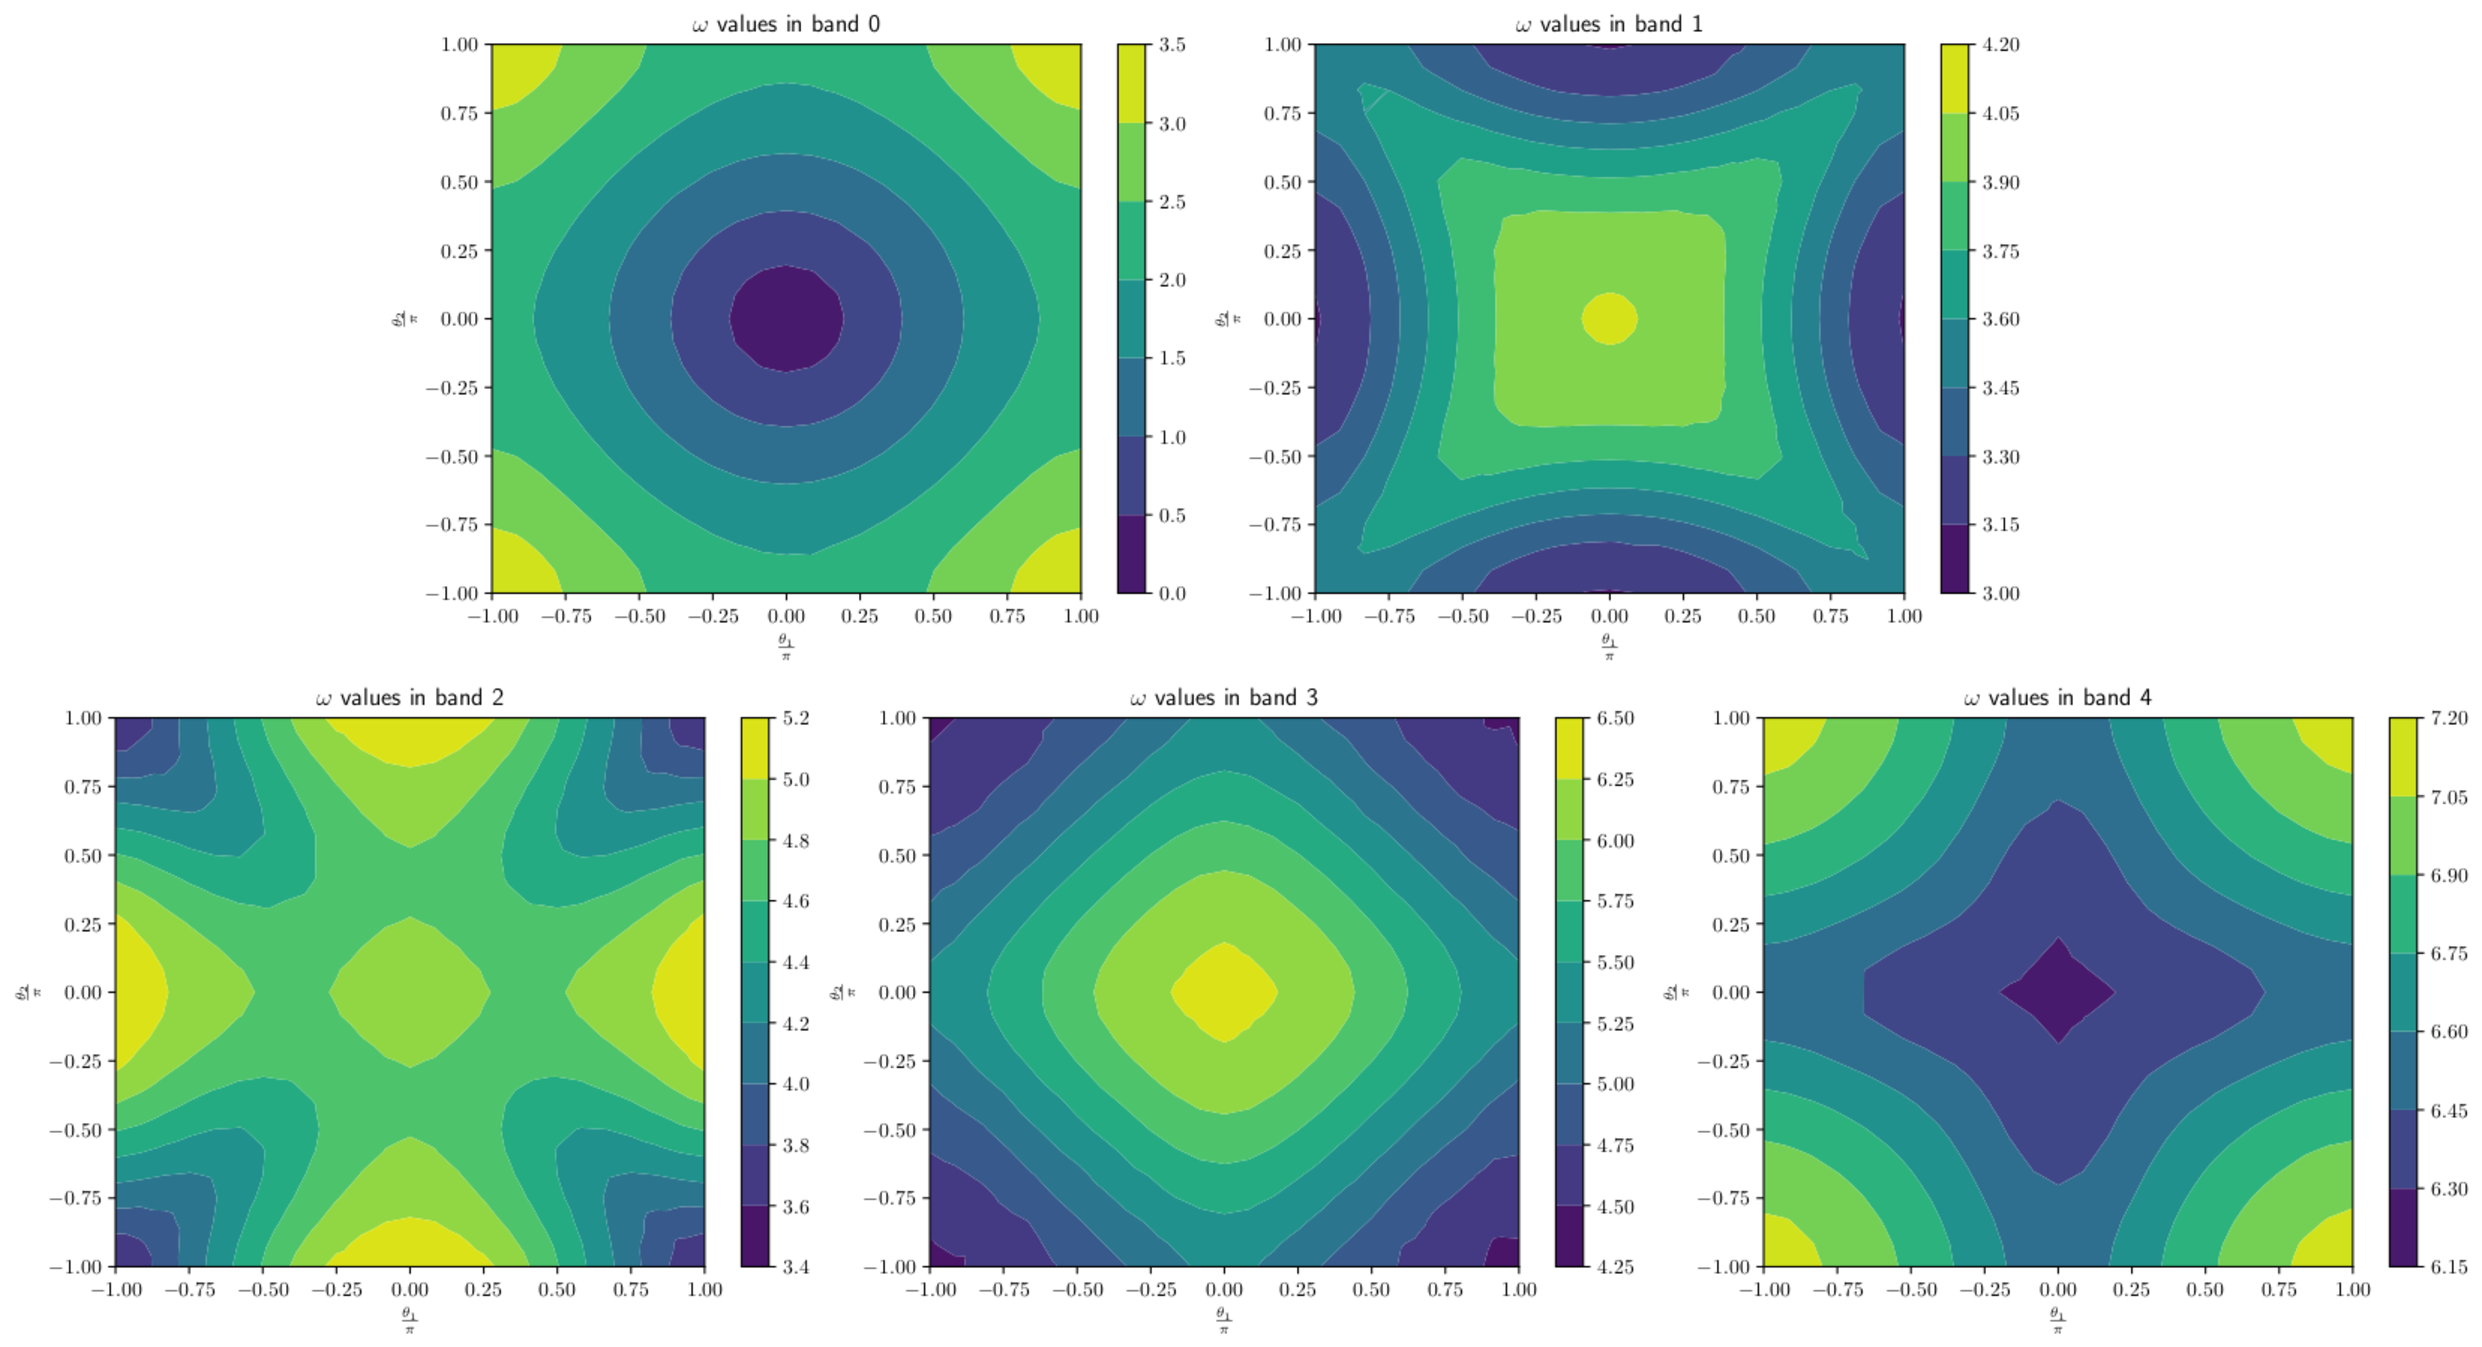
\includegraphics[width=\textwidth]{VP_2022-05-13-14-26_AllBands.pdf}
	\caption[Dispersion relations for the first 5 spectral bands of \eqref{eq:SI-WaveEqn}, computed via solution of problem \ref{prob:DiscVarProb}.]{\label{fig:VP_AllBands} The dispersion relations for the first 5 spectral bands, approximated via the problem \ref{prob:DiscVarProb}.}
\end{figure}

Although we have a method of computing the eigenvalues and eigenfunctions, we are no closer to understanding \emph{how} the presence of the skeleton and geometric contrast is affecting the problem \eqref{eq:SI-WaveEqn}.
It is also only by virtue of our analysis of the tangential gradients $\tgradSob{\ddom}{\ccompMes}$ that we are able to compute the integrals in \eqref{eq:SI-MinProblem}, and gain some insight into how we might want to approximate functions that live in $\tgradSob{\ddom}{\ccompMes}$.
In search of answers to these questions, we turn to the investigation in section \ref{sec:SI-StrongDerivation}.
We will also return to the idea of utilising a finite-element style approach to the solution of \eqref{eq:SI-WaveEqn} in our discussion in section \ref{sec:SI-Conc}.